\chapter{Results}
\label{cha:results}

\section{DAOCT}
\label{sec:results_daoct}

First to show the algorithm developed works, the example data from
\cite{moreira2018enhanced} will be used.
\todo{comentar os grafos}
\begin{figure}[H]
  \centering
  \includetikzfigure[width=\textwidth]{example/examplek1}
  \caption{DAOCT of example 2 from }
  \label{fig:exceedingLangExample}
\end{figure}

\begin{figure}[H]
  \centering
  \includetikzfigure[width=\textwidth]{example/examplek2}
  \caption{DAOCT of example 2 from }
  \label{fig:exceedingLangExample}
\end{figure}

\begin{figure}[H]
  \centering
  \includegraphics[width=0.5\textwidth]{exceedingLanguage/example/exceedingLanguage-daoct-ndaao_k2_n7.pdf}
  \caption{Cardinality of the exceeding language of the DAOCT (o) and NDAAO
    ($\times$) models. $k = 1$, and $1 \leq n \leq 7$}
  \label{fig:exceedingLangExample}
\end{figure}


Comparing the results of the \autoref{fig:exceedingLangExample}  with the
example 3 from \cite{moreira2018enhanced}, we can
observe that the exceeding language for the DAOCT model drops. This is caused by
how the acquisition works, in this work, the plant is considered a black box, so
instead of feeding the algorithm with the
paths, the raw data is given, and the paths are calculated using the first
IO\_Vector as the initial state and once this initial state is repeated other
path 
is created, resulting on 4 paths instead of 3. This change, can result in a
smaller path, with no loops, diminishing the exceeding language.


\section{Manufacture System}
\label{sec:results_system}

\begin{figure}[H]
  \centering
  \includegraphics[width=0.5\textwidth]{results/all/exceedingLanguage-daoct-ndaao_k1_n7.pdf}
  \caption{graph}
\end{figure}

\begin{figure}[H]
  \centering
  \includegraphics[width=0.5\textwidth]{results/all/exceedingLanguage-daoct-ndaao_k2-3-7_n25.pdf}
  \caption{graph}
\end{figure}

\todo{Choosing the IO\_Vector with the greatest repetition ratio as $x_0$}

\begin{figure}[H]
  \centering
  \includegraphics[width=0.5\textwidth]{results/all/best/exceedingLanguage-daoct-ndaao_k1_n7.pdf}
  \caption{graph}
\end{figure}


\begin{figure}[H]
  \centering
  \includegraphics[width=0.5\textwidth]{results/all/best/exceedingLanguage-daoct-ndaao_k2-3-7_n25.pdf}
  \caption{graph}
\end{figure}

Removing I\_MAG1EMPT and I\_MAG2EMPT

\begin{figure}[H]
  \centering
  \includegraphics[width=0.5\textwidth]{results/all-2_5/exceedingLanguage-daoct-ndaao_k1_n7.pdf}
  \caption{graph}
\end{figure}

\todo{Choosing the IO\_Vector with the greatest repetition ratio as $x_0$}

\begin{figure}[H]
  \centering
  \includegraphics[width=0.5\textwidth]{results/all-2_5/best/exceedingLanguage-daoct-ndaao_k1_n7.pdf}
  \caption{graph}
\end{figure}

As we can see, the exceedingLanguage raises




%%% Local Variables:
%%% mode: latex
%%% TeX-master: "../monografia"
%%% End:
